\chapter{Кинетическая энергия механической системы. Теорема Кёнига. Теорема об
изменении кинетической энергии механической системы. Закон сохранения
полной механической энергии.}

Кинетической энергией механической системы называется сумма кинетических энергий
всех точек, входящих в систему: \( \ds T = \sum_{k=1}^N T_k \).

\section{Теорема Кёнига}
\begin{table}[h!]
\begin{tabular}{C{.4}m{.55\textwidth}}
    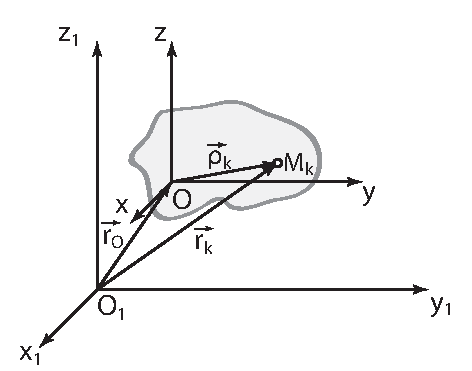
\includegraphics[width=.4\textwidth]{38_01} &
    Рассмотрим две системы отсчёта: неподвижную \( O_1x_1y_1z_1 \) и подвижную
    \( Oxyz \), поступательно движущуюся со скоростью \( \vec{v} \) относительно
    неподвижной.

    Скорость точки \( M_k \) механической системы складывается из её скорости
    относительно движущейся системы отсчёта \( \vec{v}_{kr} \) и скорости
    движущейся системы отсчёта относительно неподвижной:
    \( \vec{v}_k = \vec{v} + \vec{v}_{kr} \).

Тогда кинетическая энергия системы:
\end{tabular}
\end{table}
\vspace*{-2.5em}
\[
    T = \frac{1}{2}\sum_{k=1}^N m_k(\vec{v} + \vec{v}_{kr})^2 = \frac{1}{2}
    \sum_{k=1}^N m_k v^2 + \sum_{k=1}^N m_k\vec{v}\cdot\vec{v}_{kr} +
    \frac{1}{2}\sum_{k=1}^N m_k v_{kr}^2.
\]

Последняя сумма равна кинетической энергии относительного движения \( T_r \). Тогда:
\[
    T = \frac{1}{2}v^2\sum_{k=1}^N m_k + \vec{v}\cdot\sum_{k=1}^Nm_k\vec{v}_{kr}
    + T_r = \frac{1}{2}Mv^2 + \vec{v}\cdot\sum_{k=1}^N m_k\vec{v}_{kr} + T_r.
\]

Если начало подвижных осей \( O \) совпадает с центром масс \( C \) системы, то
\[
    \sum_{k=1}^N m_k\vec{v}_{kr} = \sum_{k=1}^N m_k\der{\rho_k}{t} = \der{}{t}
    \sum_{k=1}^N m_k\vec{\rho}_k = 0.
\]
Значит, кинетическая энергия механической системы:
\( \ds T = \frac{1}{2}Mv_C^2 + T_C \).

Кинетическая энергия материальной системы равна кинетической энергии в
поступательном движении вместе с центром масс и кинетической энергией в
относительном движении относительно центра масс.

\section{Теорема об изменении кинетической энергии}
Для каждой точки материальной системы будет справедливо следующее:
\[
    \frac{m_k v_k^2}{2} - \frac{m_k v_{0k}^2}{2} = A^e_k + A^i_k,
\]
где \( A^e_k \) и \( A^i_k \) -- работа внешних и внутренних сил соответственно.

Тогда для всей системы имеем:
\[
    \frac{1}{2}\sum_{k=1}^N m_k v_k^2 - \frac{1}{2}\sum_{k=1}^N m_k v_{0k}^2 =
    \sum_{k=1}^N A^e_k + \sum_{k=1}^N A^i_k, \quad \text{или} \quad
    T - T_0 = A^e + A^i = A.
\]
Изменение кинетической энергии материальной системы при переходе её из
начального в текущее (конечное) положение равно сумме работ на этом перемещении
всех внешних и внутренних сил, приложенных к точкам системы.

\section{Закон сохранения полной механической энергии}
Так как \( A = \varPi_0 - \varPi \) и \( T - T_0 = A \), то \( T_0 - T =
\varPi_0 - \varPi \) или \( T + \varPi = h \), где \( h = T_0 + \varPi_0 =
\const \).
Таким образом, если система движется под действием только консервативных сил, то
сумма кинетической и потенциальной энергий сохраняет постоянное значение.

\newpage
